\section{\S~Assessment Study}

\begin{frame}{Predictability}
  \begin{figure}
    \centering
    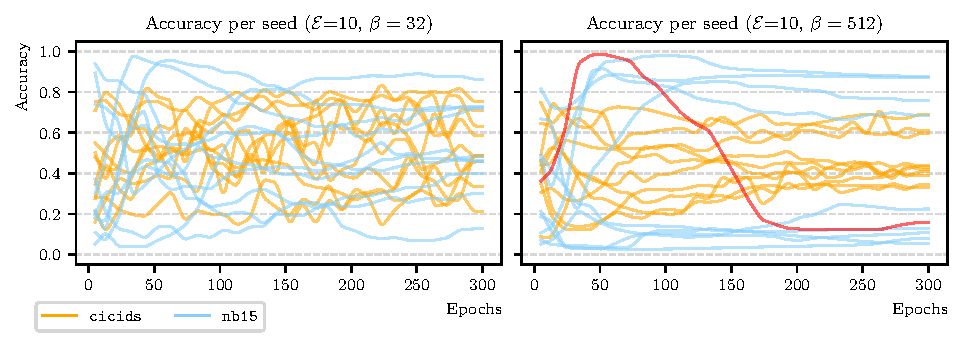
\includegraphics[width=0.8\textwidth]{figures/thesis/assessment/accuracy_per_seed.pdf}
    \caption{Accuracy of a FIDS under attack, across different random seeds.}
  \end{figure}
\end{frame}

\begin{frame}{Impact on attack propagation}
  \begin{figure}
    \centering
    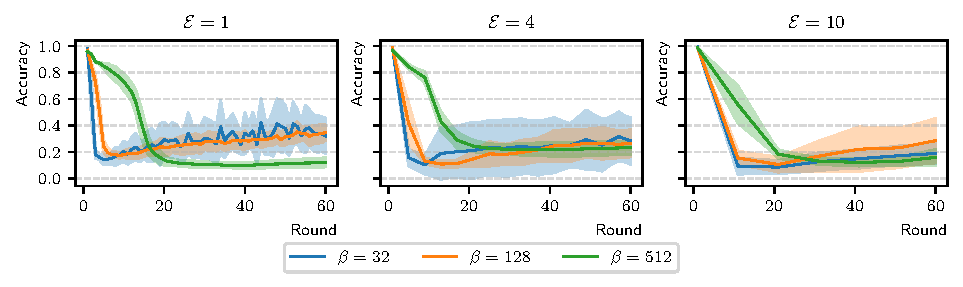
\includegraphics[width=0.8\textwidth]{figures/thesis/assessment/hyperparams-late-icdcs.pdf}
    \caption{Accuracy across rounds for different batch sizes.}
  \end{figure}
\end{frame}

\begin{frame}{Similarity-based Mitigation against Heterogeneity}

  \begin{columns}
    \begin{column}{.45\textwidth}
      \begin{itemize}[<+->]
        \item Known technique to detect poisoning attacks~\autocite{tolpegin_DataPoisoningAttacks_2020}.
        \item High heterogeneity makes it harder to detect attackers.
      \end{itemize}
    \end{column}

    \begin{column}{.55\textwidth}
      \begin{figure}
        \centering
        \foreach \i in {1,...,3}{%
          \includegraphics<\i>[width=\textwidth,trim={1cm 3cm 1cm 3cm},clip]{figures/thesis/assessment/similarity-untargeted-colluding-cicids-\i.pdf}%
        }
        \caption{PCA projection of the gradients in 2D (CICIDS).}
      \end{figure}
    \end{column}
  \end{columns}

  \footcite*{tolpegin_DataPoisoningAttacks_2020}

\end{frame}

\section{\S~Neural-symbolic AI}

\begin{frame}{IA neuro-symbolique\normalfont\normalsize~(\logic)}
  \begin{figure}
    \centering
    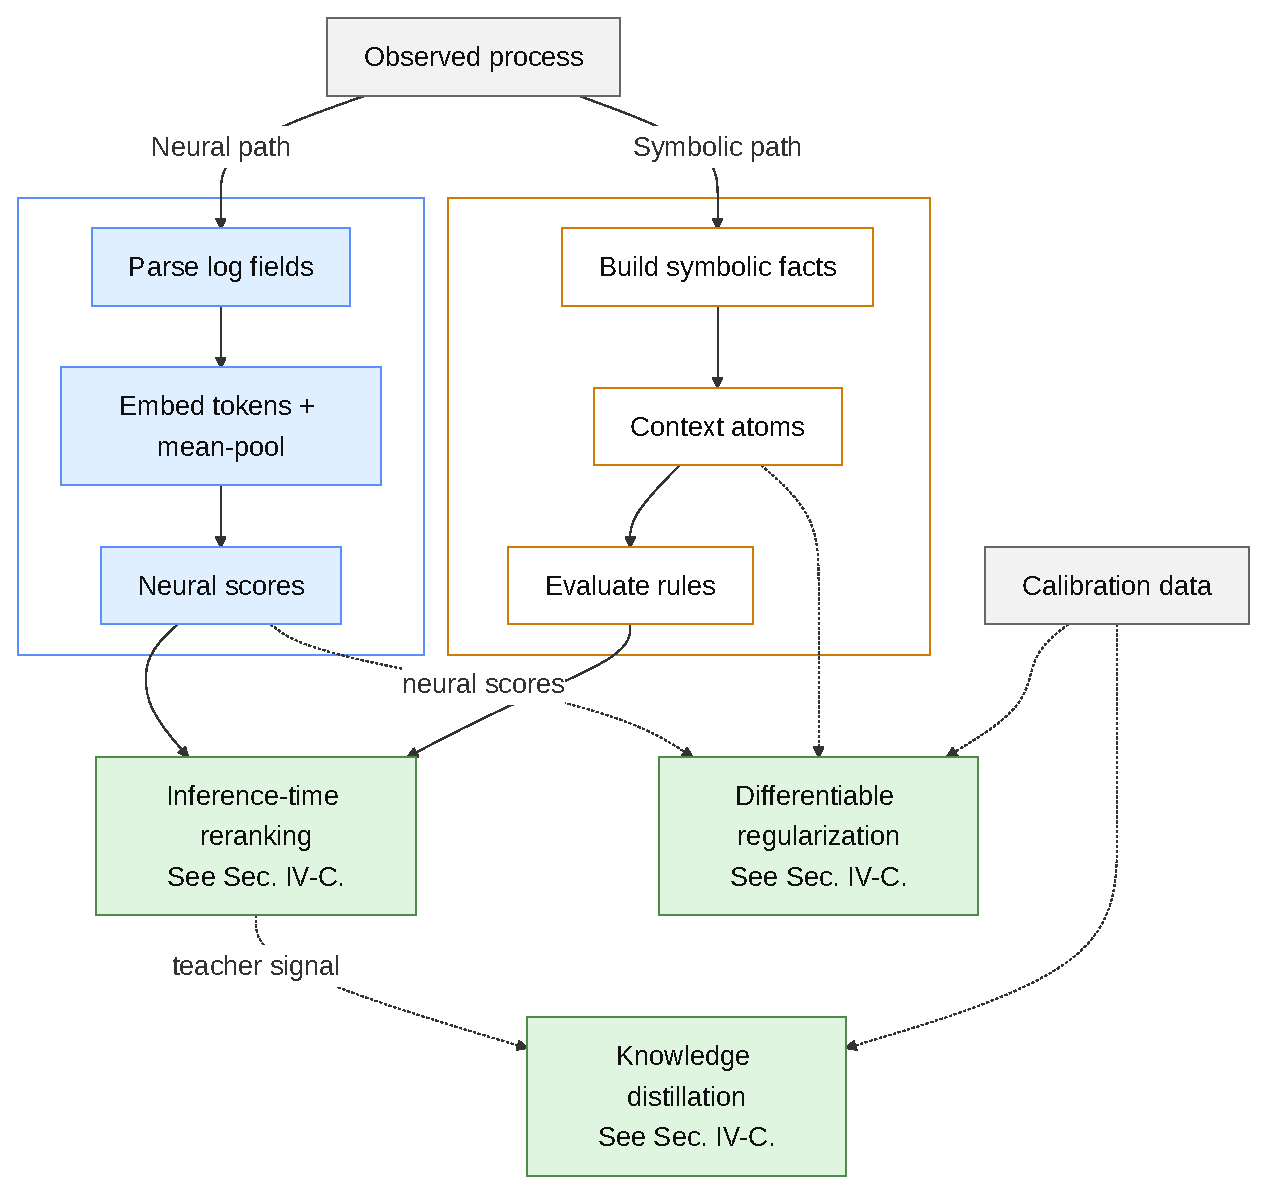
\includegraphics[width=0.5\textwidth]{figures/backup/nesy-detection.pdf}
    \captionof{figure}{Différentes intégrations neuro-symboliques.}
  \end{figure}
\end{frame}

\begin{frame}{IA neuro-symbolique\normalfont\normalsize~(\logic)}
  \centering
  \begin{table}
    \centering
    \caption{Fixing misclassification issues in CasinoLimit by adding contextual logic rules using Scallop.
    Macro-F1 on the targeted instances.}
    \small
    \begin{tabular}{llll}
      \toprule
      \textbf{Row} & \textbf{Ping (\texttt{ligolo-ng})} & \textbf{Grep (\texttt{linpeas.sh})} & \textbf{Combined} \\
      \midrule
      Baseline & 0.423277 & 0.423277 & 0.423277 \\
      Logic at inference & 0.455895 (+7.71\%) & 0.488943 (+15.51\%) & 0.521561 (+23.22\%) \\
      KL Distillation & 0.438017 (+3.48\%) & 0.533949 (+26.15\%) & 0.555552 (+31.25\%) \\
      Logic at training & 0.444519 (+5.02\%) & 0.560168 (+32.34\%) & 0.618868 (+46.21\%) \\
      %Relabelling & 0.444132 (+4.93\%) & 0.585468 (+38.32\%) & 0.697962 (+64.89\%) \\
      \bottomrule
    \end{tabular}
  \end{table}
\end{frame}

\begin{frame}{\texttt{Scallop}}
  \begin{figure}
    \centering
    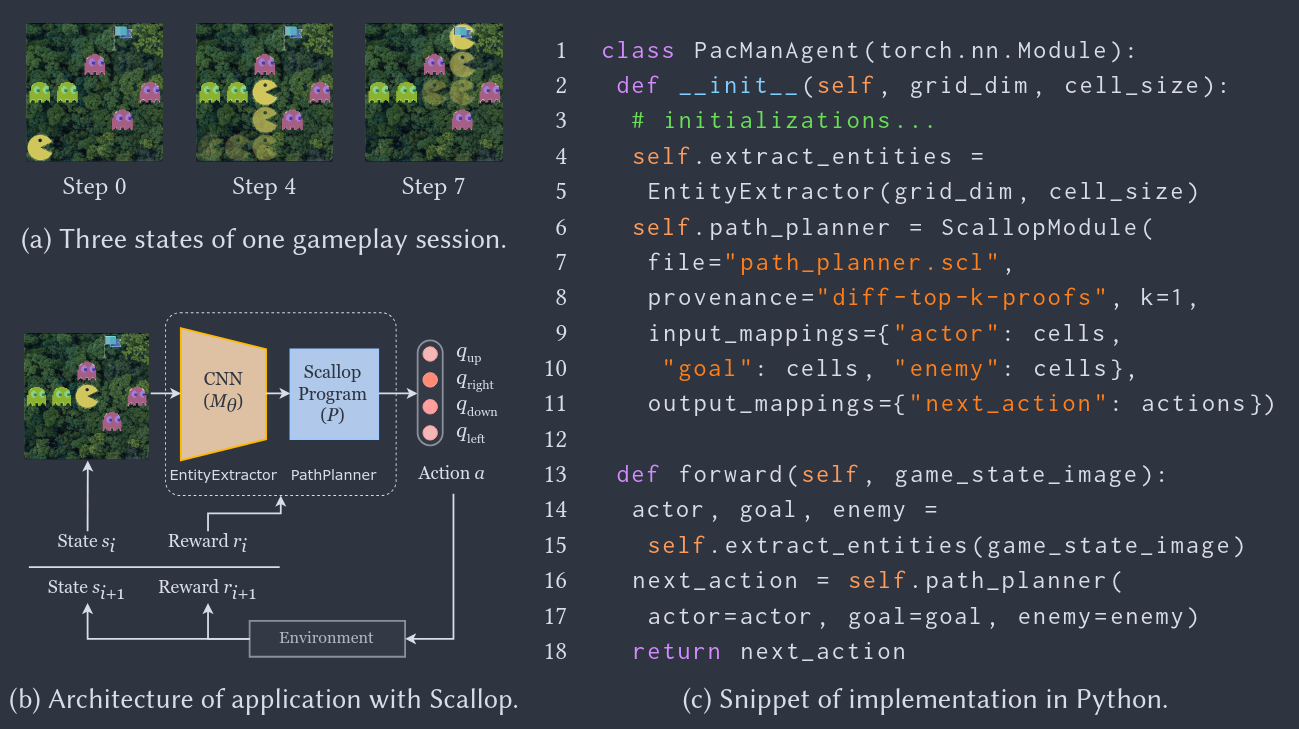
\includegraphics[width=0.75\textwidth]{figures/postdoc/scallop_appendix.png}
    \caption{Scallop~\footcite{huang_ScallopProbabilisticDeductive_2021}.}
  \end{figure}
\end{frame}

\begin{frame}{\texttt{DeepProbLog}}
  \begin{figure}
    \centering
    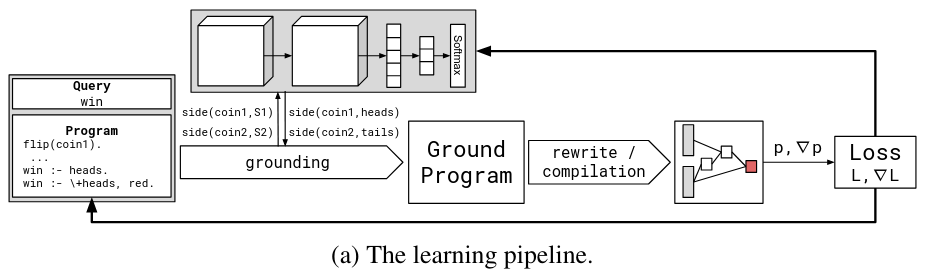
\includegraphics[width=0.8\textwidth]{figures/postdoc/deepproblog_appendix.png}
    \caption{DeepProbLog~\footcite{manhaeve_DeepProbLogNeuralProbabilistic_2018}.}
  \end{figure}
\end{frame}

\section{\S~\tt FedITN\_gen}

\input{sections/feditn/approach.tex}